\chapter{序論}
\label{chapter:introduction}

本章では,本研究の実施に至った背景を説明し,対象とする課題を明確にする.

%------------------------------------------------------------------------
\section{本研究の背景}
  現在,都市には多種多様な視覚情報が溢れている.
  人々はこのような情報が密集している都市空間から,提示されている情報を手がかりに意思決定を行っている.
  都市空間において人々が店舗を探す際,飲食店や衣料店などといった店舗の種類を判別するための手がかりの1つに,看板が挙げられる.
  例えば,人々が飲食店を探す場合,飲食店の看板や案内はユーザにとって必要な情報であり,それ以外の衣料店などの情報は不要な情報に分類できる.
  このように,多くの人々は看板を手がかりに街中で情報探索を行っている.

  また,近年,日本を訪れる観光客は増加しつつある.
  日本政府観光局によると,2012年に8,358,105人であった訪日観光客は,2017年には28,691,073人と,3倍を超えて増加している\cite{JNTO:2018}.
  こうした訪日外国人の増加にも関わらず,店舗の看板などは多言語で記載されているとは限らない.
  例として,日本語の看板に店舗名がローマ字で併記されていたとしても,日本語が分からなければ,それが店の名前であることも分からない.
  その上,外国人観光客は日本人の多くが常識として持っている情報を持っていないことも多く,外国人にとってはどの店がどのようなサービスを行っているか,クレジットカードでの決済はできるかなどの情報を看板から得ることは容易ではない.
  そのため,日本人に与えられている情報をただ翻訳して伝えるだけでは不十分である\cite{Hayashida:2005}.

\section{街中における検索行為}
  街中においてユーザが周囲の店舗の情報を検索する際,現状ではスマートフォンなどの携帯端末を用いて,位置情報や看板に書かれている店舗名などを手がかりに周辺の検索を行うことで,求める条件に合致した店舗を探している.
  その店で享受できるサービスの種類を知る上で,看板は重要な役割を果たしているが,図\ref{figure:kabukicho}のように看板が密集している地域においては,一軒一軒の店舗情報を検索する必要があり,このような情報を速やかに得ることは容易ではない.
  そのため,目的とする情報の探索に少なからず時間を要してしまう.
  特に,初めて訪れる場所など,慣れていない地域でユーザが看板などの視覚情報を探す場合,特定の情報を素早く見つけることは困難である.
  Google Map\footnote{\url{https://www.google.com/maps}(2019/1/14存在確認)}などの地理情報システムには,住所から地図上の位置を特定する機能がある.
  しかし,位置情報を用いるのみではユーザが実際に見ている看板や標識などの現実世界上における正確な位置まで提示できず,ユーザがいる環境と検索行為とが分断されており,その環境から目的の店舗を探す手間が残されている.
  そのため,探索する看板が未知であるものや,目立たないものである場合,大量に存在する他の視覚情報に紛れて,見つけることができない可能性があり,目的の店舗を発見することは容易ではない.

  また,外国人観光客の場合,自身の目の前にある店舗が自身の求める条件に合致するかスマートフォンで検索しようとしても,言語障壁によりどのように検索して良いか分からない場合がある.
  さらに,位置情報を用いて周辺の店舗情報を検索し,条件に合う店舗が見つかったとしても,その店舗の看板に書かれている文字を読むことができなければ,多数ある店舗の中から目的の店舗を発見することは容易ではない,
  そのため,結局ガイドマップに記載されている店舗など,限られた選択肢から選択せざるを得ない状況にある.
  店舗側が看板を多言語化することや,QRコードを用いて多言語で情報を配信する手法もあるが,様々な言語圏からの来訪者すべてに対応するには限界があり,このような手法では店舗側の負担も大きい.

\section{本研究の目的}
\label{section:purpose}
  本研究では,繁華街や商店街などユーザの周囲に店舗が多数存在する地域において,(1)視覚情報の識別性を向上させ,ユーザが目的の店舗を見つけるのに要する時間を短縮させること,
  (2)ユーザが慣れていない地域や周囲の文字が読めない状況であっても,目の前にある店舗の情報を直感的かつ簡単に取得できるようにすること,の2点を目的とする.

  (1)を実現するために,先行研究\cite{Fujita:2013}で提案されたユーザにとって不要な情報を目立たなくさせる手法を改良し,必要な情報に付加情報を重畳表示する提示手法を提案した.さらに,全天球カメラで撮影した画像内において,条件に合う店舗を探索するプロトタイプを実装した.これにより,視覚情報が密集している地域において,ユーザが迷うことなく目的の店舗を発見できるようになることが期待される.
  (2)を実現するために,スマートフォンを店舗の看板にかざすことで,地理情報システムのデータベースに登録されている店舗情報を取得し,カメラ映像上に店舗情報を重畳表示するシステムを提案し,特定の地域を対象とした実環境で利用できるプロトタイプを実装した.これにより,言語障壁があっても,ユーザが目の前の店舗でどのようなサービスが得られるのかを知ることができるようになり,求める条件に合致した店舗を直感的に選択できるようになることが期待される.

  本稿ではこれらの提案システムの優位性を検証するために従来手法と比較したユーザ実験を行い,その結果について述べる.

  \begin{figure}[tb]
    \centerline{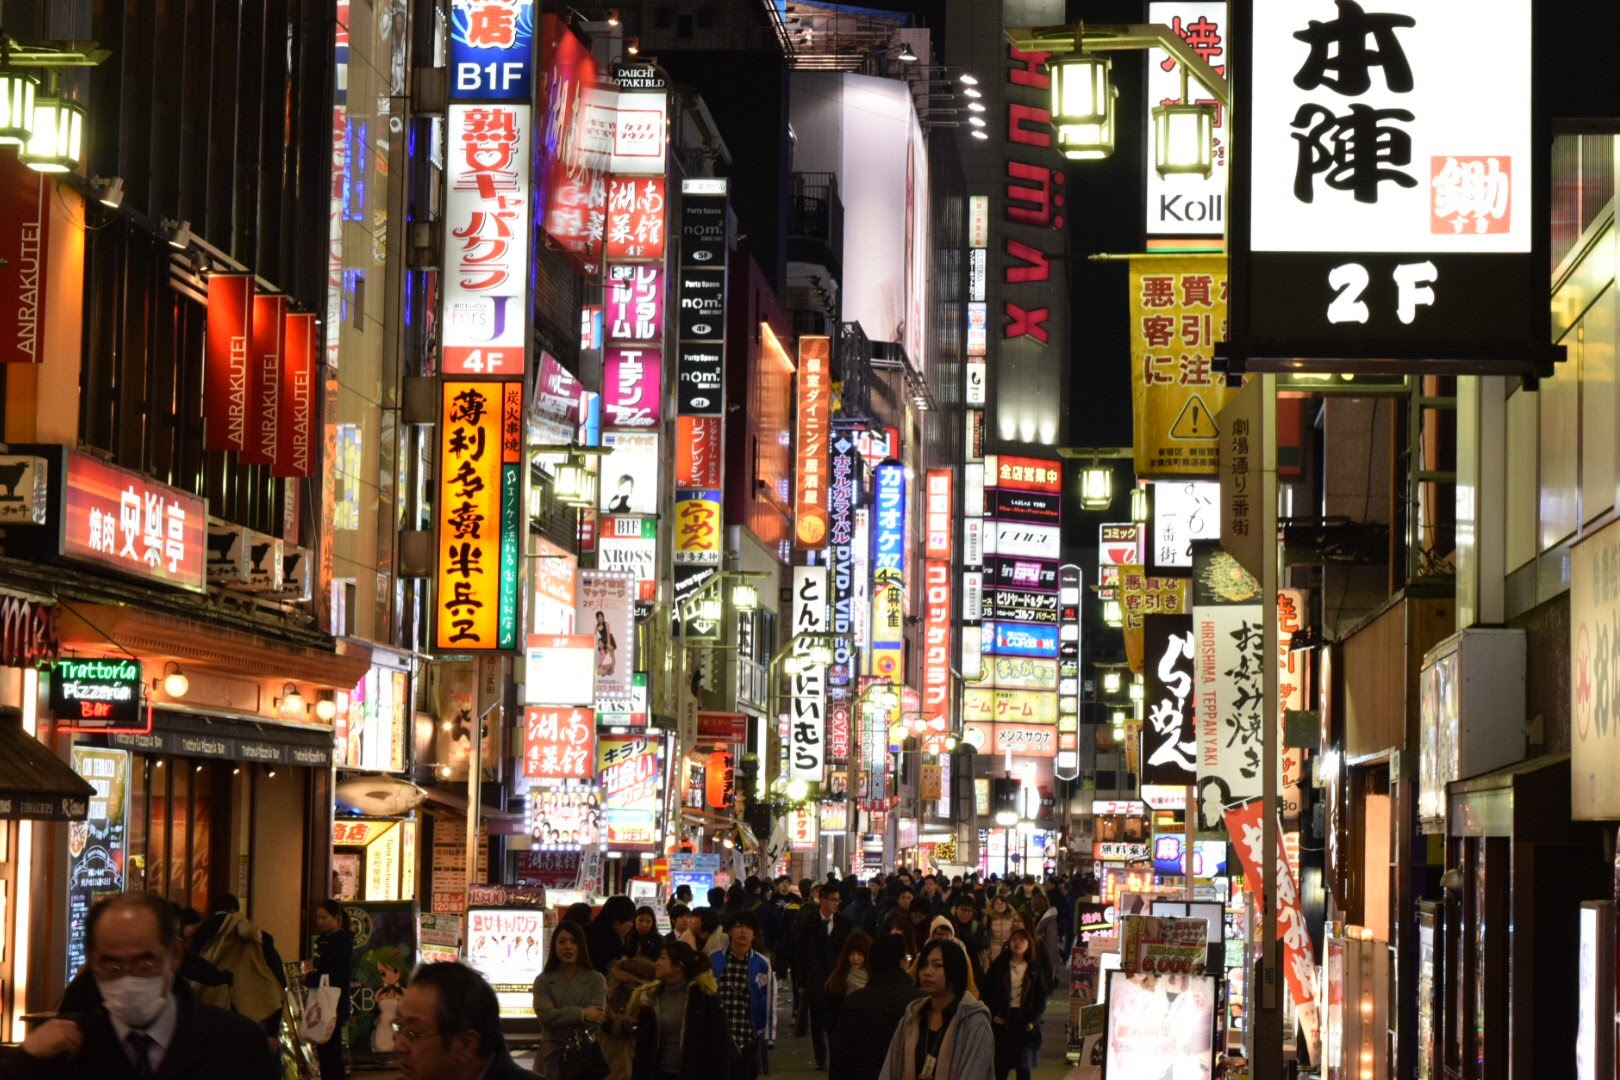
\includegraphics[width=\columnwidth, clip]{kabukicho.jpg}}
    \caption{密集する看板情報(新宿・歌舞伎町にて撮影)}
    \label{figure:kabukicho}
  \end{figure}
